% %%%%%%%%%%%%%%%%%%%%%%%%%%%%%%%%%%%%%%%%%%%%%%%%%%%%%%%%%%%%%%%%%%%%%
% %% Background %%
% Kernels and Algorithms
% %%%%%%%%%%%%%%%%%%%%%%%%%%%%%%%%%%%%%%%%%%%%%%%%%%%%%%%%%%%%%%%%%%%%%

% rank / OP / IP / Gust / tile / tiling / partial outputs / partial sums / intersections

\section{Algorithms for Dense and Sparse Matrix Multiplication}
\label{sec:bg:algos}

The accelerators described in this paper address sparse \acrshort{mv} and \acrshort{mm}.
For \acrshort{mv} we use the notation $A(M,K) \times b(K) = c(M)$ and for \acrshort{mm} the notation $A(M,K) \times B(K,N) = C(M,N)$.
The \emph{rank} $K$ is the \emph{common rank} between the two inputs.

The existence of different \emph{ranks} allows several algorithmic possibilities to compute matrix multiplication: the \acrfull{ip} algorithm, the \acrfull{op} algorithm and \acrlong{gust}'s (\acrshort{gust}) algorithm~\cite{Faddeev1981_InnerOuter, Gustavson1978_GustAlgo}.
In all cases, the matrix $A$ is traversed sequentially.
The three algorithms, however, impose different access patterns for $B$ (or $b$) and $C$ (or $c$).
Indeed, in many cases, they have to be accessed multiple times, as discussed in the following sections.

\subsubsection{Inner-Product Algorithm}

The \acrlong{ip} algorithm~\cite{Faddeev1981_InnerOuter} is an intuitive way to calculate a matrix multiplication because it follows the loop order of the mathematical formulas~(\ref{eq:bg:MVinner}) and~(\ref{eq:bg:MMinner}) for \acrshort{mv} and \acrshort{mm}, respectively.

\begin{equation}
    \forall i \in \ldb0, M-1\rdb, \; c_{i} = \sum_{k = 0}^{K-1} A_{i,k} \times b_{k}
    \label{eq:bg:MVinner}
\end{equation}

\begin{equation}
    \forall (i, j) \in \ldb0, M-1\rdb \times \ldb0, N-1\rdb, \; C_{i, j} = \sum_{k = 0}^{K-1} A_{i,k} \times B_{k,j}
    \label{eq:bg:MMinner}
\end{equation}

The \emph{common rank} $K$ is the inner-most loop of the algorithm (see Algorithms~\ref{alg:bg:MVinner} and~\ref{alg:bg:MMinner}).
The output $C$ (or $c$) is updated sequentially, but the $B$-matrix (or $b$-vector) will be entirely read $M$ times.
In the context of sparse matrices, the reads of $B$ (or $b$) are conditioned by the non-zero elements of $A$, which requires indirect accesses.
If $B$ (or $b$) is also sparse, the algorithm needs to perform \emph{intersections} between the non-zero elements in the rows of $A$ and the columns of $B$ (or in the $b$-vector) (see Section~\ref{sec:bg:hwchallenges}).
In Algorithm~\ref{alg:bg:MMinner}, exchanging $M$ and $N$ simply causes the output to be updated \emph{column-wise}.

\begin{figure}
    \begin{minipage}[t]{0.49\linewidth}
        \begin{algorithm}[H]
        \caption{\acrlong{mv} \acrlong{ip} Algorithm}
        \label{alg:bg:MVinner}
        \For{$i \in \ldb 0, M-1 \rdb$}{
            \For{$k \in \ldb 0, K-1 \rdb$}{
                $c_{i} \acc A_{i,k} \times b_{k}$
            }
        }
        $ $\\
        $ $
        \end{algorithm}
    \end{minipage}
    \hfill
    \begin{minipage}[t]{0.49\linewidth}
        \begin{algorithm}[H]
        \caption{\acrlong{mm} \acrlong{ip} Algorithm}
        \label{alg:bg:MMinner}
        \For{$i \in \ldb 0, M-1 \rdb$}{
            \For{$j \in \ldb 0, N-1 \rdb$}{
                \For{$k \in \ldb 0, K-1 \rdb$}{
                    $C_{i,j} \acc A_{i,k} \times B_{k,j}$
                }
            }
        }
        \end{algorithm}
    \end{minipage}
\end{figure}

\subsubsection{Outer-Product Algorithm}

The \acrlong{op} algorithm~\cite{Faddeev1981_InnerOuter} has the opposite \emph{rank} loop order than the \acrlong{ip}.
It changes nothing mathematically except that the computation is separated into two phases.
First, during the \emph{multiply} phase, we compute several \emph{partial outputs} (\emph{POs}) consisting of the \emph{partial sums} $A_{j,k} \times b_{k}$, then during the \emph{merge} phase, we accumulate all the \emph{POs} to form the final $C$-matrix (or $c$-vector).
Algorithms~\ref{alg:bg:MVouter} and~\ref{alg:bg:MMouter} show that the \emph{common rank} $K$ is the outer-most loop.
Inverting $M$ and $N$ affects whether the output $C$ (or $c$) is updated by rows or by columns, but has no influence on the indirect accesses to the inputs.

\begin{figure}
    \begin{minipage}[t]{0.49\linewidth}
        \begin{algorithm}[H]
        \caption{\acrlong{mv} \acrlong{op} Algorithm}
        \label{alg:bg:MVouter}
        \For{$k \in \ldb 0, K-1 \rdb$}{
            \For{$i \in \ldb 0, M-1 \rdb$}{
                $c_{i} \acc A_{i,k} \times b_{k}$
            }
        }
        $ $\\
        $ $
        \end{algorithm}
    \end{minipage}
    \hfill
    \begin{minipage}[t]{0.49\linewidth}
        \begin{algorithm}[H]
        \caption{\acrlong{mm} \acrlong{op} Algorithm}
        \label{alg:bg:MMouter}
        \For{$k \in \ldb 0, K-1 \rdb$}{
            \For{$i \in \ldb 0, M-1 \rdb$}{
                \For{$j \in \ldb 0, N-1 \rdb$}{
                    $C_{i,j} \acc A_{i,k} \times B_{k,j}$
                }
            }
        }
        \end{algorithm}
    \end{minipage}
\end{figure}

With \acrlong{op}, the $B$-matrix (or $b$-vector) is read sequentially.
This algorithm necessitates the generation of $K$ \emph{POs}.
Moreover, in the context of sparse input matrices, the \emph{PO} element updates are conditioned by the non-zeros elements of both inputs.
Thus, a \emph{partial sum} could potentially be zero, reducing the number of \emph{PO} element updates, and making them non-sequential.
If the output $C$ (or $c$) is stored in a \emph{sparse format}, then it is necessary to repeatedly access and update each \emph{partial sum}.

\subsubsection{Gustavson's Algorithm}

As the \acrshort{mm} algorithm has three \emph{ranks} instead of two for \acrshort{mv}, there is a third ordering, known as \acrlong{gust}'s algorithm~\cite{Gustavson1978_GustAlgo} where the \emph{common rank} $K$ is the middle loop (see Algorithm~\ref{alg:bg:MMgustavson}).
With this approach, the output is computed row-by-row with \emph{PO}-rows generated and accumulated for each output $C$-row.

\begin{figure}
    \centering
    \begin{minipage}[t]{0.49\linewidth}
        \begin{algorithm}[H]
        \caption{\acrlong{mm} \acrlong{gust}'s Algorithm}
        \label{alg:bg:MMgustavson}
        \For{$i \in \ldb 0, M-1 \rdb$}{
            \For{$k \in \ldb 0, K-1 \rdb$}{
                \For{$j \in \ldb 0, N-1 \rdb$}{
                    $C_{i,j} \acc A_{i,k} \times B_{k,j}$
                }
            }
        }
        \end{algorithm}
    \end{minipage}
\end{figure}

With this algorithm, updates of the $C$-rows are sequential, but, in the dense case, the $B$-matrix is entirely read $M$ times and $K$ \emph{PO}-rows of size $N$ are generated.
In the context of sparse matrices, the selection of the rows in $B$ is indirect, however, within a row the accesses are sequential.
The \emph{intersection} operations are only needed for the $B$-rows and not each element.
The \emph{PO}-rows can be accumulated before computing the next $C$-row.
For this algorithm, exchanging $M$ and $N$ causes the three matrices to be accessed \emph{column-wise} instead of \emph{row-wise}.

\subsubsection{Algorithms Comparison}

Note that these algorithms are available in dense as well as in sparse \acrshort{mv} and \acrshort{mm} multiplications.
In sparse, the above algorithms (from \ref{alg:bg:MVinner} to \ref{alg:bg:MMgustavson}) have the same behavior from a software point-of-view, but need adjustments to traverse a \gls{spFormat} instead of a dense matrix.

TODO

\begin{table}
    \centering
    \caption{Comparison of Matrix Multiplication Algorithms}
    \footnotesize
    \begin{tabular}{|>{\centering\arraybackslash}m{1.5cm}|| *{3}{>{\arraybackslash}m{4.2cm}|}}
        \hhline{-||---}
        & \textbf{\acrfull{ip}} & \textbf{\acrfull{op}} & \textbf{\acrfull{gust}} \\
        \hhline{=::===}
        \textbf{A$(M, K)$} \newline \textbf{Accesses} & $\bullet$ read $N$ times\hyperlink{fn3}{$^{\mathrm{1}}$} \newline $\bullet$ \emph{row-wise} \newline $\bullet$ sequential & $\bullet$ read once \newline $\bullet$ \emph{column-wise} \newline $\bullet$ sequential & $\bullet$ read once \newline $\bullet$ \emph{row-wise} \newline $\bullet$ sequential \\
        \hhline{-||---}
        \textbf{B$(K, N)$} \newline \textbf{Accesses} & $\bullet$ read $\overline{nnz_{r}}(A) \times M$ times \newline $\bullet$ \emph{column-wise} \newline $\bullet$ not sequential & $\bullet$ read $\overline{nnz_{c}}(A)$ times\hyperlink{fn4}{$^{\mathrm{2}}$} \newline $\bullet$ \emph{row-wise} \newline $\bullet$ sequential & $\bullet$ read $\overline{nnz_{r}}(A)$ times\hyperlink{fn4}{$^{\mathrm{2}}$} \newline $\bullet$ \emph{row-wise} \newline $\bullet$ sequential within rows \\
        \hhline{-||---}
        \textbf{C$(M, N)$} \newline \textbf{Accesses} & $\bullet$ sequential \newline $\bullet$ generated \emph{row-wise} & $\bullet$ generated without specific structure \newline $\bullet$ $K$ \emph{POs} produced (each \emph{PO} has $nnz_{c}(A) \times nnz_{r}(B)$ non-zero elements) & $\bullet$ generated \emph{row-wise} \newline $\bullet$ for each row, $nnz_{r}(A)$ \emph{PO} rows produced (each \emph{PO} rows has $nnz_{r}(B)$ non-zero elements) \\
        \hhline{-||---}
        \multicolumn{4}{l}{\hypertarget{fn3}{$^{\mathrm{1}}$}In the case of \acrshort{mv} multiplication, $N=1$.} \\
        \multicolumn{4}{l}{\hypertarget{fn4}{$^{\mathrm{2}}$}Average number of non-zero entries in the rows/columns of $A$.}
    \end{tabular}
    \label{tab:AlgosCompSum}
\end{table}

\subsection{Tiling}
\label{sec:bg:tiling}

The \emph{tiling} process~\cite{Grunbaum1987_Tiling} consists in matrix partitioning: a matrix may be divided into \emph{tiles}, non-overlapping sub-matrices.
In other words, this method consists of adding \emph{ranks} to delimit the \emph{tiles}, and thus adding loop iterations in the kernel algorithm.

\emph{Tiling} methods allow to locally reduce the dimensions of data and thus to adapt the working set to the size of the local memory~\cite{Lam1991_Tiling}, particularly when the matrix has a structure with denser regions.
Tiling can also increase parallelism opportunities.
Software optimizations for sparse matrix computation, such as OSKI~\cite{Vuduc2005}, are based on \emph{tiling}.
In previous sections, the study of the \algo{IP}, \algo{OP} and \algo{Gust} algorithms highlighted the influence of \emph{rank} ordering on the sequentiality and data movement, and thus, adding intermediate \emph{ranks} with \emph{tiling} breaks the regularity of pure \algo{IP} or \algo{OP} algorithms, requiring additional hardware support (see Section~\ref{sec:bg:hwchallenges}).

For example, let us consider the $A$-matrix in Figure~\ref{fig:bg:tiling_ex} which is divided into four tiles (one level of \emph{tiling}).
For a SpMV, two new \emph{ranks} appear for a total of four \emph{ranks}: $M_1$ and $K_1$ allow \emph{tile} selection and $M_2$ and $K_2$ allow data access within a \emph{tile}.
Thus, we could decide to apply an \algo{OP} on \emph{tiles} and conversely an \algo{IP} within \emph{tiles}, mixing-up the pros and cons of these two algorithms at different \emph{rank} levels.
In the case of the example in Figure~\ref{fig:bg:tiling_ex}, the upper-left $A$-\emph{tile} (red) is evaluated first, sequentially updating the upper tile of the $c$-vector in an \algo{IP} manner.
The lower-left $A$-\emph{tile} (yellow) is then computed the same way. At this point, \emph{intersections} have been done with only the upper $b$-\emph{tile}, and $c$ has been updated sequentially.
The two next $A$-\emph{tiles} (green, then blue) will compute \emph{intersections} with the lower $b$-\emph{tile} and update the entire $c$-vector sequentially, showing the \algo{OP} characteristic of having \emph{POs} to \emph{merge}, two in this case.
% add ref to algo

\begin{figure}
    \centering
    \begin{minipage}[t]{0.28\linewidth}
        \begin{figure}[H]
            \centering
            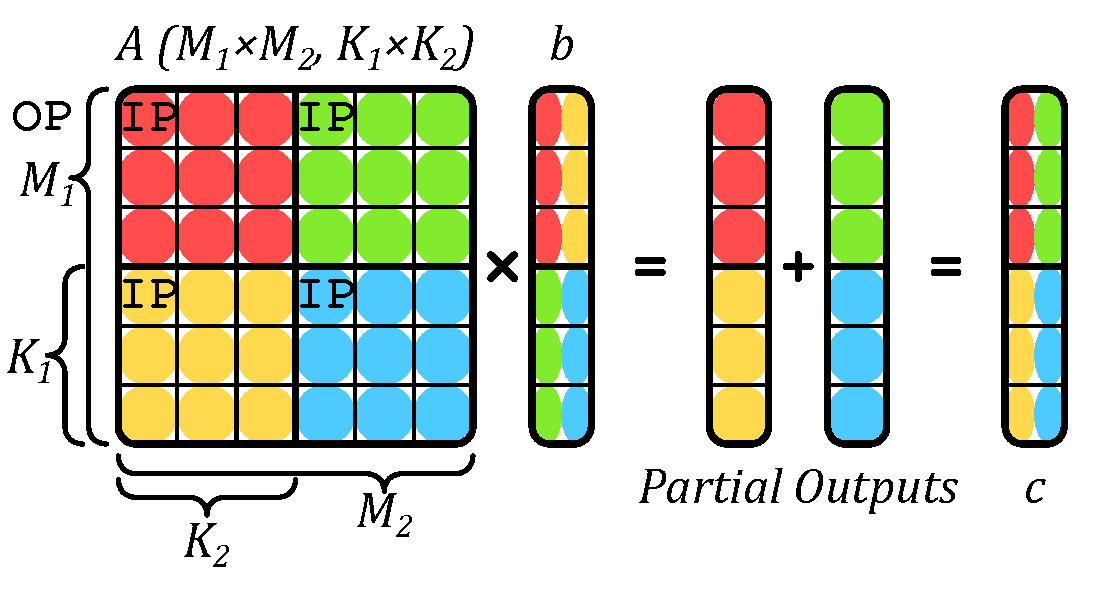
\includegraphics[width=\linewidth]{Chapter_Background/Figures/PDF/TilingExample.pdf}
            \caption{An Example of \Gls{tiling} on \acrshort{spmv}}
            \label{fig:bg:tiling_ex}
        \end{figure}
    \end{minipage}
    \hfill
    \begin{minipage}[t]{0.60\linewidth}
        \bigskip\bigskip
        \begin{algorithm}[H]
        \caption{\acrlong{mv} Algorithm with Custom \Gls{tiling} of Figure~\ref{fig:bg:tiling_ex}}
        \label{alg:bg:tiling_ex}
        \For{$k_1 \in \ldb 0, K_1-1 \rdb$}{
            \For{$i_1 \in \ldb 0, M_1-1 \rdb$}{
                \For{$i_2 \in \ldb 0, M_2-1 \rdb$}{
                    \For{$k_2 \in \ldb 0, K_2-1 \rdb$}{
                        $i \gets i_1 \times M_2 + i_2$\\
                        $k \gets k_1 \times K_2 + k_2$\\
                        $c_i \acc A_{i, k} \times b_k$
                    }
                }
            }
        }
        \end{algorithm}
    \end{minipage}
\end{figure}

Note that in case of \emph{tiling}, the $A$-matrix is no longer read sequentially, which can be problematic if it is stored in a classical \emph{sparse format} like \emph{CSR} that is specifically made for \emph{row-wise} accesses.
Custom \emph{sparse formats} adapted for \emph{tiling} can be used \cite{Im2004_TilingBCSR}, but this requires a preprocessing conversion.